\chapter{Rozbor hry}
\section{Herní deska}
Herní deska má vždy tvar šesticípé hvězdy, nezávisle na počtu hráčů. Existují dvě verze desek, lišící se v počtu herních polí a kamenů přidělovaných hráčům. Podle jedné verze by měla deska obsahovat celkem 192 polí \cite{zapletal}, s tím že každému hráči je přiděleno patnáct kamenů (s výjimkou případu, kdy probíhá hra šesti hráčů, v takovém případě zůstává nejdelší řada ve výchozím trojúhelníku hráče prázdná a každý hráč má tedy pouze deset kamenů). Herní desku v této verzi můžeme vidět na obrázku číslo \ref{fig:VerzeHerniDesky}.

\begin{figure}
	\centering
	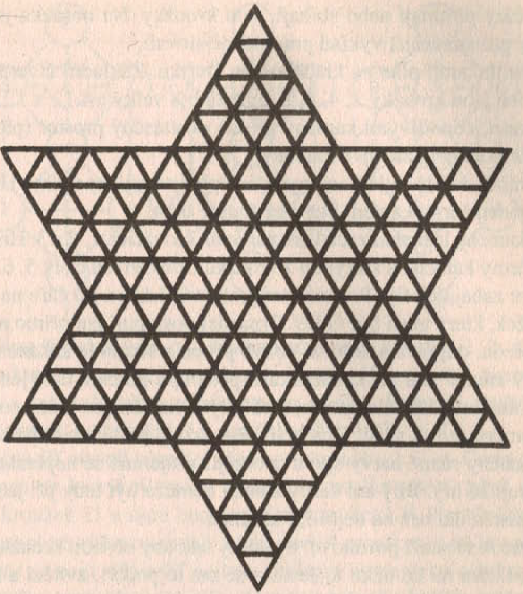
\includegraphics[width=0.4\textwidth]{Figures/VerzeHerniDesky.png}
	\caption{Verze herní desky obsahující 192 polí \cite{zapletal}}
    \label{fig:VerzeHerniDesky}
\end{figure}

Zmíněná verze herní desky již ale není v dnešní době příliš používána. I v této práci je využita druhá verze desky, ve které je obsaženo 121 polí, a každému hráči je přiděleno bez ohledu na počet hráčů vždy deset kamenů. Tato herní deska obsahuje 17 sloupců a 13 řádků. U žádných dvou sousedních polí na desce nelze vytvořit vertikální úsečku spojující jejich středy -– každé pole je totiž horizontálně umístěno přesně mezi pole nalézající se nad ním nebo pod ním. Vytvoření horizontálních úseček spojující středy dvou sousedních polí je oproti tomu umožněno. Samotná herní deska je~v~naší aplikaci uložena v okně \lstinline$HraForm$ v panelu pojmenovaném \lstinline$herniPanel$. Ten slouží k práci s~vytvořenými herními poli.

\section{Herní pole}
\label{sec:HerniPole}
Jako první je vytvořeno pole nalézající se z pohledu uživatele na samotném vrcholu trojúhelníku, jedná se o pole s nejnižší $y$-ovou souřadnicí ze všech polí. U tohoto pole bylo zvoleno vhodné odsazení od hranic panelu, vzorec pro určení odsazení na $x$-ové ose je uveden v rovnici (\ref{eq:leveOdsazeni}), na $y$-ové je rovno hodnotě 13px. Poloha všech ostatních polí se odvíjí od tohoto pole, protože poloha každého pole je přímo závislá na poloze předchozího vytvořeného pole.

\begin{equation}
leveOdsazeni = \frac{1}{2}(sirkaPanelu - sirkaPole)
\label{eq:leveOdsazeni}
\end{equation}

$X$-ová a $y$-ová souřadnice daného pole jsou uloženy v proměnných \lstinline$poz_X_He$ a \lstinline$poz_Y_He$. Mezi další parametry každého pole patří jeho šířka a výška, ty jsou uloženy v proměnných \lstinline$sirkaPole$~a~\lstinline$vyskaPole$ a jejich hodnota činí 35px. Mezi všemi poli je ve všech směrech rozestup o hodnotě 5px, pro usnadnění je proto vytvořená proměnná \lstinline$posun$ označující vzdálenost mezi dvěma sousedními poli, a to horizontálně i vertikálně, rovnající se součtu rozměru pole a rozestupu mezi poli, tedy 40px. Znázornění souřadnic všech polí je k dispozici na obrázku číslo \ref{fig:SouradnicePoli}. Posledním parametrem pole je \lstinline$jeAktivni$, podle kterého určujeme, jestli může být pole během dané hry některým hráčem využito.

Samotné vytvoření pole probíhá v cyklu, kdy je během každé iterace vytvořeno vždy jedno pole. Během každé iterace je hodnota \lstinline$poz_X_He$ zvyšována o \lstinline$posun$, čímž je zajištěno rozmístění polí na $x$-ové ose. Pokaždé, kdy se má vytvořit nový řádek polí, je hodnota \lstinline$poz_Y_He$ zvýšena také o \lstinline$posun$ a hodnota \lstinline$poz_X_He$ je nastavena na $x$-ovou polohu prvního pole v daném řádku. 

\begin{figure}
	\centering
	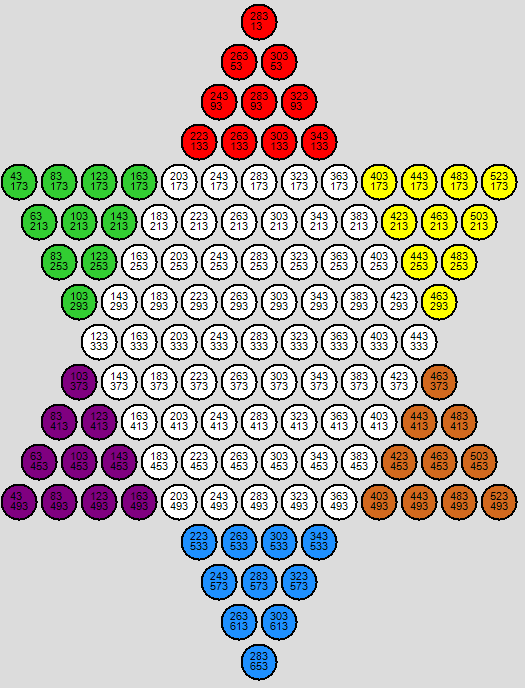
\includegraphics[width=0.7\textwidth]{Figures/SouradnicePoli.png}
	\caption{Souřadnice herních polí}
    \label{fig:SouradnicePoli}
\end{figure}

\section{Možné výsledky hry}
\label{sec:MozneVysledkyHry}
Po konci každého tahu je zkontrolováno, jestli se během daného tahu nepodařilo některému z hráčů přemístit všechny své kameny do daného cílového trojúhelníku. Hra může z pohledu lidského hráče skončit jedním ze čtyř výsledků:
\begin{description}
\item [výhra]  -- nastane v případě, že se lidskému hráči podaří přemístit všechny své kameny do cílového trojúhelníku jako prvnímu ze všech hráčů. Příklad lidským hráčem vyhrané hry můžeme vidět na obrázku číslo \ref{fig:Vyhra}.
\item [prohra]\index{prohra}  -- nastane v opačném případě než výhra, tedy tehdy, když se některému z počítačových hráčů povede přemístit všechny své kameny do daného cílového trojúhelníku dříve než lidskému hráči. Příklad lidským hráčem prohrané hry\index{prohra!hry} můžeme vidět na obrázku číslo \ref{fig:Prohra}.
\item [remíza]  -- relativně neobvyklý výsledek hry, nastává v případě, kdy se dvěma a více hráčům podaří přemístit všechny své kameny do daného cílového trojúhelníku během stejného tahu.~V~takovém případě hráč nevyhrál ani neprohrál, ale remizoval. Příklad takového výsledku hry můžeme vidět na obrázku číslo \ref{fig:Remiza}
\item [kontumace]\index{kontumace}  -- také se jedná o nepříliš častý výsledek hry, do hry je přidána jako ochrana proti taktice blokování. Nastává v případě, kdy hráč přemístil své kameny do všech volných polí cílového trojúhelníku a do zbývajících je nemůže přemístit výhradně z důvodu, že jsou obsazena hráčem, pro kterého je tento trojúhelník výchozím. Pro udělení kontumace\index{kontumace} je nutné splnění následující podmínky: součet kamenů patřících hráči, pro kterého je daný trojúhelník výchozím, nalézajících se ve třech polích nejbližších k cípu hvězdy a kamenů patřících hráči, pro kterého je daný trojúhelník cílovým, nalézajících se v celém trojúhelníku, musí být roven 10. V takovém případě už totiž hráč, který v trojúhelníku začínal, nemůže trojúhelník opustit bez toho, aniž by hráč, pro kterého je trojúhelník cílovým, neprovedl pro sebe nevýhodné tahy, kterými by mu uvolnil cestu k opuštění trojúhelníku. Grafické znázornění situací, při kterých nastává kontumace\index{kontumace}, je k dispozici na obrázku číslo \ref{fig:Kontumace}. Rozmístění kamenů ve třech polích nejbližších k cípu hvězdy je při kontumaci irelevantní, v potaz je bráno pouze splnění nebo nesplnění podmínky, jestli se kameny v těchto třech polích nacházejí. Stejně tak není brán ohled na polohu kamenů patřících hráči, pro kterého je trojúhelník cílový, nacházejících se mimo cílový trojúhelník, ohled je brán pouze na jeho kameny umístěné v cílovém trojúhelníku. Podmínky pro kontumaci jsou kontrolovány po každém tahu stejně jako podmínky pro vítězství. Pokud dojde ke kontumaci, je danému hráči přidělena kontumační výhra. Dá se ji tedy brát jako typ výhry, nicméně při ukončení hry je uvedeno, že hráč vyhrál kontumačně.
\end{description}
Po ukončení hry je uživateli ukázána zpráva o vítězícím hráči, uživatel se poté může vrátit do hlavního menu nebo může provést restartování hry, čímž vytvoří novou hru se stejnými parametry.

\begin{figure}
	\centering
	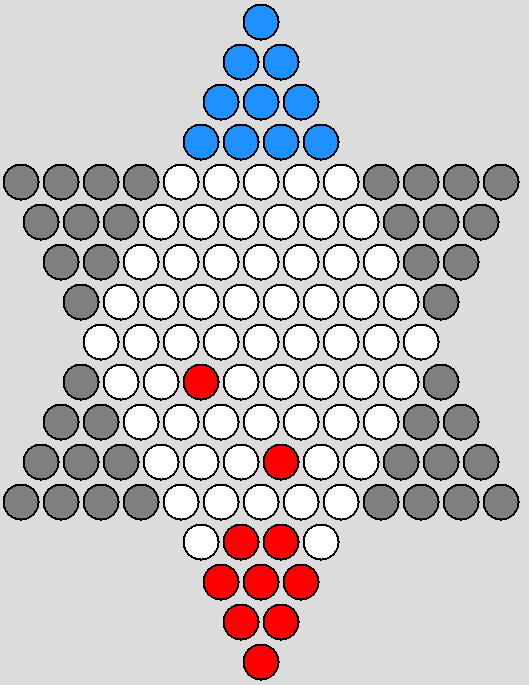
\includegraphics[width=0.4\textwidth]{Figures/Vyhra.png}
	\caption{Lidským hráčem vyhraná hra}
    \label{fig:Vyhra}
\end{figure}

\begin{figure}
	\centering
	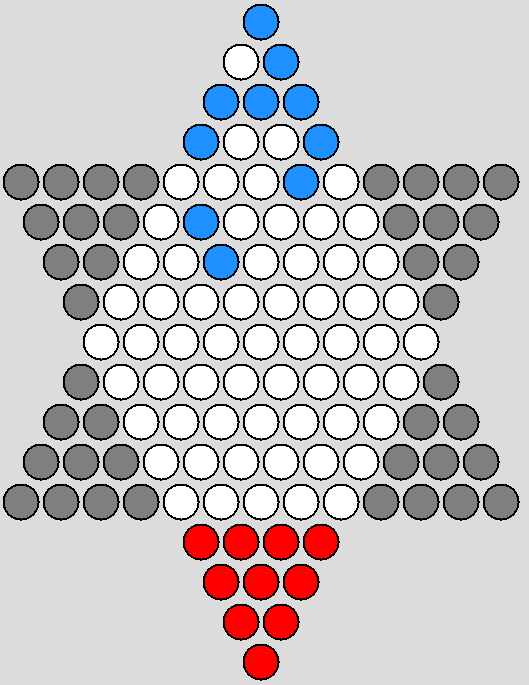
\includegraphics[width=0.4\textwidth]{Figures/Prohra.png}
	\caption{Lidským hráčem prohraná hra}
    \label{fig:Prohra}
\end{figure}

\begin{figure}
	\centering
	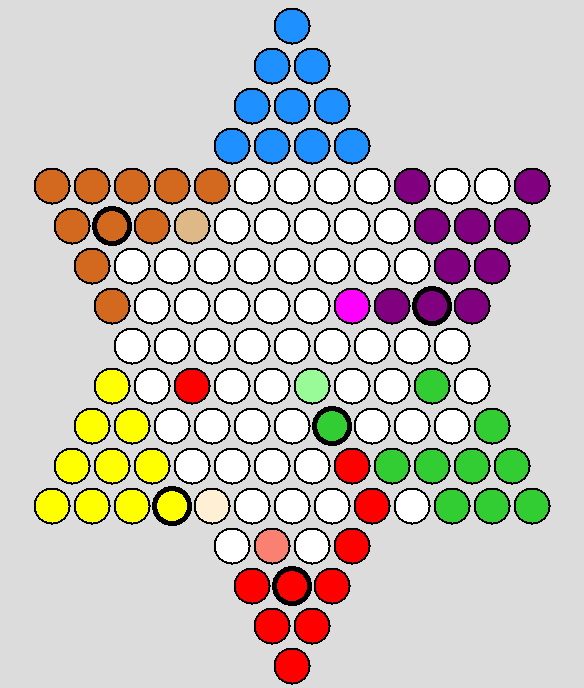
\includegraphics[width=0.4\textwidth]{Figures/Remiza.png}
	\caption[Příklad hry, ve které došlo k remíze]{Příklad hry, ve které došlo k remíze – během stejného tahu splnil podmínky výhry jak modrý (lidský) hráč, tak žlutý (počítačový) hráč}
    \label{fig:Remiza}
\end{figure}

\begin{figure}
	\centering
	\subfloat[Situace, kdy hráči v jeho výchozím trojúhelníku zbyl 1 kámen\label{fig:Kontumace1}]
	{
		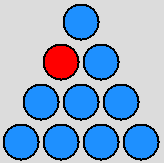
\includegraphics[width=0.35\textwidth]{Figures/Kontumace1.png}
	}
	\hspace{3em} % make more space
	\subfloat[Situace, kdy hráči v jeho výchozím trojúhelníku zbyly 2 kameny\label{fig:Kontumace2}]
	{
		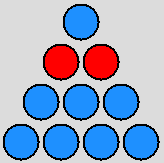
\includegraphics[width=0.35\textwidth]{Figures/Kontumace2.png}
	}
	\hspace{3em} % make more space
	\subfloat[Situace, kdy hráči v jeho výchozím trojúhelníku zbyly 3 kameny\label{fig:Kontumace3}]
	{
		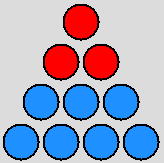
\includegraphics[width=0.35\textwidth]{Figures/Kontumace3.png}
	}
	\caption[Příklady situací, při kterých nastává kontumace]{Příklady situací, při kterých nastává kontumace\index{kontumace} (s ohledem na počet kamenů, který hráči zbyl v jeho výchozím trojúhelníku)}
	\label{fig:Kontumace}
\end{figure}
\endinput